\documentclass[12pt]{book}
\usepackage{diffyqssetupUB}
\usepackage{hyperref}

\begin{document}

%extra material {Notes about these notes}

\subsection {Computing with Python}

In the exploration and application of differential equations, a lot can be accomplished by writing a little computer code.
You can manipulate mathematical formulas, 
generate approximate but accurate solutions of equations numerically, and 
create graphical representations of differential equations and their solutions.
We show you how, using Python. Python is a modern programming language that is free, relatively easy to learn,
and very versatile. For simplicity of installation, we recommend the Anaconda distribution of Python, 
which can be downloaded from 
\href{https://www.anaconda.com/distribution/\#download-section}{https://www.anaconda.com/distribution/\#download-section}, 
choosing the Python 3.7 version for your operating system.
There you can also find the simple installation instructions. 

We also recommend writing and
running your code in Jupyter Notebook which is supplied with the Anaconda distribution, and which 
provides a convenient and elegant environment within your web-browser 
where you can do your computations, display your results, and write a report around them.

To make a few important tasks simple, we provide code to draw slope fields (\Chapterref{fo:chapter}), and
vector fields and phase portraits (\Chapterref{sys:chapter} and \Chapterref{nlin:chapter}). 
This code is available at 
\newline
\href{https://raw.githubusercontent.com/UBmath/306/master/resources306.py}{https://raw.githubusercontent.com/UBmath/306/master/resources306.py}, 
and should be saved 
{\color{blue} as file resources306.py }
in the same folder as the notebook in which you want to use it.
{\color{teal}BH Links open a text file and no instructions what to do.
Better if link opens a box offering to save file as resources306.py. JR How to do that in latex?
BH I tried \htref{URL download} which
didn't work under Overleaf, but that might be
an Overleaf issue- will try LaTeX directly}
{\color{red}Perhaps the easiest}
{\color{blue}One} way to accomplish this is to run the following Python code in your Jupyter notebook.
If you copy-and-paste code from the PDF of this book, you should check that the indentation remains correct: 
in Python, indentation matters.


\begin{small}
\begin{verbatim}
import requests
url = 'https://raw.githubusercontent.com/UBmath/306/master/resources306.py'
r = requests.get(url)
with open('resources306.py','w') as f:
    f.write(r.text)
\end{verbatim}
\end{small}

\parbox[c]{3.1in}{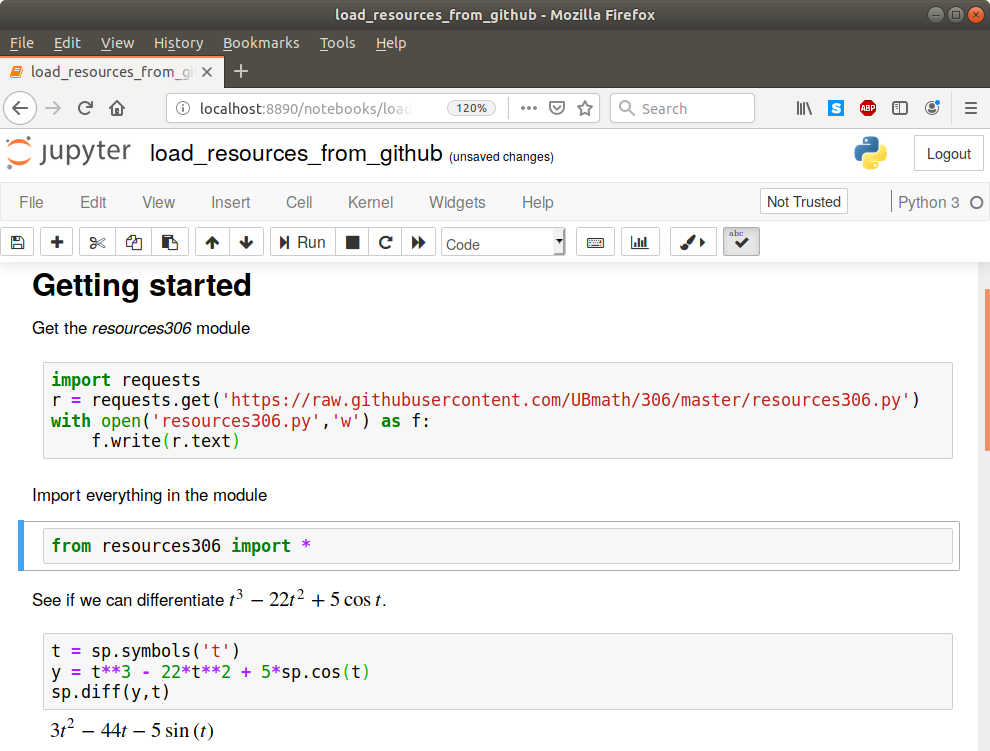
\includegraphics[width=4.0in]{additional_figures/Introduction_to_differential_equations__getting_started}}

{\color{teal}BH changed includegraphics width from 4.0 to 6.0 to try to match font size inside graphic to font size in other graphics}

%extra material {Introduction to differential equations}

\subsection {Checking and plotting solution formulas with Python}

We can check that formulas really are solutions of a differential equations using the symbolic
computation capabilities of \emph{sympy}. This is especially useful in complicated cases
where we may not totally trust our own hand-computations. In the screenshot on the next page, we recheck the results of \ref{solutions:subsection}.
See \sectionref{notes:section} for how to obtain the "resources306" module.


{\color{teal}JR: BH's suggestion followed in revised figure. OK to delete red above. BH done}

Solution plots like the one on the next page can also be created using \emph{numpy} instead of \emph{sympy}, as shown below.
The idea is to generate a sequence of points along the graph and join them with straight line segments. 
We use several hundred points so that the curve looks smooth. In the example (a),
we plot the curve $y = e^{-2t}$ for $t$ between -1 and 2. In example (b), we plot a
family of curves indexed by the parameter $c$ which runs over the values $\{4, 5, 6, ..., 15\}$.
There are many options for modifying and decorating such plots: to find out how, ask Google "matplotlib how to add title to plot", etc.

\noindent (a) 
\begin{small}
\begin{verbatim}
# the following line imports sympy as sp, numpy as np, matplotlib.pyplot as plt
from resources306 import *
t = np.linspace(-1,2,200)
plt.plot( t, np.exp(-2*t) );
plt.grid()
\end{verbatim}
\end{small}

\noindent (b)
\begin{small}
\begin{verbatim}
t = np.linspace(0,0.02,100)
for c in np.linspace(4,15,12):
        plt.plot( t, 13/(1-(1-13/c)*np.exp(91*t)) )
plt.xlim(0,.02)
plt.ylim(0,20)
\end{verbatim}
\end{small}


(a)\parbox[c]{2.6in}{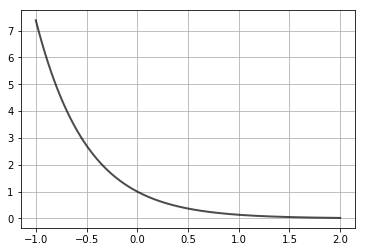
\includegraphics[width=2.5in]{additional_figures/Introduction_to_differential_equations__single_curve}}
(b)\parbox[c]{2.6in}{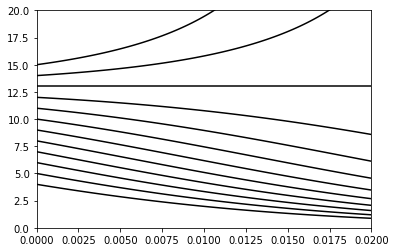
\includegraphics[width=2.5in]{additional_figures/Introduction_to_differential_equations__family_of_curves}}
\newpage  % hack to avoid excessive spacing on the page
\parbox[c]{7.5in}{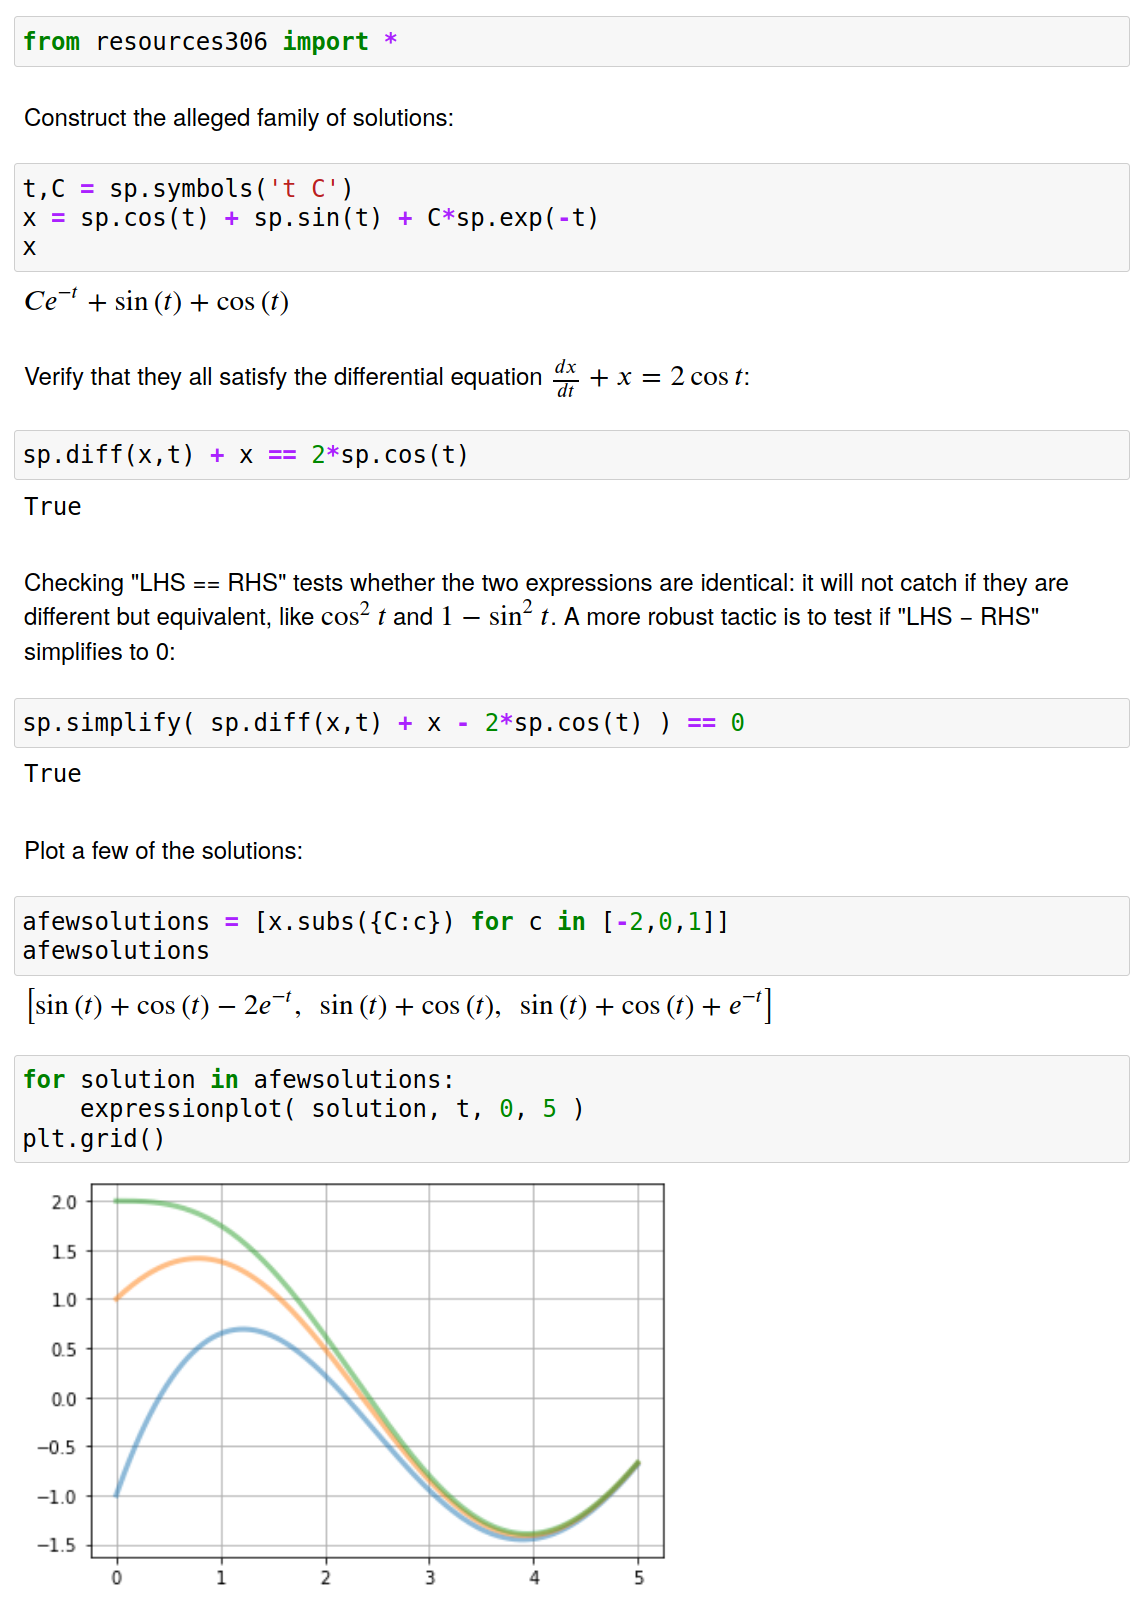
\includegraphics[width=6.5in]{additional_figures/checking_solutions.png}}

\newpage % tweak 1/9/2020

\end{document}

